\chapter{Evaluation des Systems}
\label{sec:evaluation}
Nach erfolgreicher Implementierung des DAB/DAB+ Transceivers folgt in diesem Abschnitt eine Evaluation des Systems. Für eine grundsätzliche Verifikation wird der Empfänger gegen das DAB+ Ensemble eines lokalen Radiosenders in einer realen Übertragung getestet. In der Simulation wird der Transceiver anschließend auf sein Verhalten und seine Robustheit bei verschiedenen Übertragungskanälen untersucht. \\
Für quantitative Aussagen stellt die \ac{BER} ein gängiges Gütekriterium zur Bewertung der Übertragungsqualität des physikalischen Kanals dar. Die \ac{BER} allein ist jedoch kein ausreichendes Maß für die vom Nutzer subjektiv empfundene Qualität des Empfangssignals. Sowohl im FIC als auch im MSC entscheidet letzlich ein CRC darüber, ob ein FIB beziehungsweise ein MPEG Frame korrekt ist und es dementsprechend weiterverarbeitet oder verworfen wird. Das Audiosignal wird, im Gegensatz zu FM, bei gestörter Übertragung nicht verrauschter, sondern die Ausfallrate, auch \ac{PER} genannt, steigt. Deshalb ist es sinnvoll, die Fehlerrate dieser Pakete über die CRCs als Gütekriterium für eine praktische bzw. subjektive Übertragungsqualität zusätzlich zur Bitfehlerrate heranzuziehen.\\

Die Performanz des Systems hängt von vielen Faktoren ab. Die Konzeption der Systemarchitektur entscheidet über die grundlegenden Eigeschaften des Systems und ist durch den ETSI DAB Standard \cite{etsi:dab_main} festgelegt. Ein weiterer wesentlicher Faktor ist das Design der Synchronisation. Es ist nicht im Standard spezifiziert und deshalb stark von der jeweiligen Implementierung abhängt.

\section{Verifikation des Empfängers}
Der Empfänger wird gegen ein lokales DAB+ Ensemble des Südwestrundfunks (SWR) verifiziert. Die Sendestation ist in ca. 10 km Entfernung und sendet mit einer \ac{ERP} von etwa 1 kW \cite{web:wattkopf_sender}. Der Empfang findet im Gebäude und ohne Bewegung des Empfängers statt. Es wurden insgesamt 3 Empfängerkonfigurationen getestet:

\begin{figure} [h]
\begin{tabular}{l | c | c}
Hardwarekonfiguration & SNR & subjektive Empfangsqualität \\
\hline
USRP B210 mit DAB-Stabantenne & $\approx 50$ dB & komplett störungsfrei \\
USRP B210 mit Teleskopantenne & $\approx 28$ dB & komplett störungsfrei \\
RTL-SDR mit DVB-T kleiner Stabantenne & $\approx 18$ dB & gestört
\end{tabular}
\caption{getestete Hardwarekonfigurationen und deren Ergebnisse}
\label{tab:hardware}
\end{figure}

Durch den erfolgreichen Empfang des SWR DAB+ Ensembles ist der Empfänger verifiziert. Die SNR Werte spiegeln wie zu erwarten die Eignung der jeweiligen Antenne für den DAB Empfang wider. Der hohe Qualitätsunterschied der SDR-Geräte ist bei der reinen SNR Messung nicht vollständig berücksichtigt, wirkt sich aber im weiteren Verlauf der Synchronisations- und Decodierungskette auf die Empfangsqualität aus.\\
Zur subjektiven Empfangsqualität seien zwei Anmerkungen gemacht: Die subjektive Audioqualität der DAB+ Übertragung ist im Vergleich zu FM wesentlich besser; dies kommt jedoch nur bei der Verwendung eines hochwertigen Lautsprechers oder Kopfhörer zum Tragen. Bei kostengünstigen Lautsprechern ist ein Qualitätsunterschied kaum hörbar. Bei sehr schlechter Empfangsqualität fallen einzelne DAB+ Audioframes aus und unterbrechen dadurch den Audiostream für die Dauer eines Superframes von $120 ms$. Auch wenn die restlichen Audioframes komplett fehlerfrei und rauschfrei sind, ist in diesem Fall das sehr verrauschte aber unterbrechungslose FM Audiosignal angenehmer für den Hörer. Eine mögliche Verbesserung dieser subjektiven Empfindung kann durch weiches Aus- und Einblenden vor bzw. nach einem Frameausfall erreicht werden. Diese Methode wird in einigen kommerziellen DAB+ Radios bereits eingesetzt und erzielt den gewünschten Effekt.


\section{AWGN Kanal}
Der \ac{AWGN} Kanal ist das einfachste hier verwendete Kanalmodell. Der Kanal addiert bei der Übertragung weißes, gaußsches Rauschen auf das Sendesignal.
\begin{equation}
R(t) = S(t) + N(t) \quad \text{mit} \quad N(t) \sim \mathcal{C}\mathcal{N}(0,\,\sigma^{2})
\end{equation}

\subsection{Bitfehlerrate}
Die simulierte Bitfehlerrate des DAB Systems wird über dem SNR gemessen, indem bei bekannter Signalleistung $P_s = 1$ W die Rauschleistung entsprechend dem SNR eingestellt wird. Um aussagekräftige Ergebnisse über die Performanz einer digitalen Übertragung zu erhalten ist nach \cite{snr:sklar2001digital} die Bitenergie im Verhältnis zur Rauschleistungsdichte $\text{E}_b/\text{N}_0$ ein sinnvolleres Gütemaß als das SNR, da Energie Bits überträgt, und nicht Leistung.
Die Umrechnung von SNR zu $\text{E}_b/\text{N}_0$ ergibt:
\begin{equation}
\begin{aligned}
\frac{E_b}{N_0} &= \frac{P_s}{N} \cdot \frac{B}{R} \quad \text{mit} \quad P_s=1,\; B=1,\; N=\sigma^2 \\
&= \frac{1}{\sigma^2} \cdot \frac{1}{R} \\
&= \frac{1}{\sigma^2} \cdot \frac{1}{\frac{K}{N_{Tr\ddot{a}ger}} \cdot \log_2 (M) \cdot \frac{T_S}{T_G+T_S}}
\end{aligned}
\end{equation}
Die Bitrate $R$ ergibt sich aus den Systemparametern. Symbolratenverluste entstehen durch $K=1536$ belegten von insgesamt $N_{Tr\ddot{a}ger}=2048$ verfügbaren OFDM Unterträgern. Die redundante Wiederholung von QPSK Symbolen im Cyclic Prefix verkleinert die effektive Symbolrate weiter. Jedes QPSK Symbol transportiert dabei $\log_2 (4) = 2$ Bits. Damit ergibt sich das folgende Verhältnis von SNR zu $\text{E}_b/\text{N}_0$ in dB:
\begin{equation}
\frac{E_b}{N_0} = \text{SNR} \; - \; 10\cdot \log_{10} \left(\frac{1536}{2048} \cdot 2 \cdot \frac{2048}{504+2048} \right) \approx \text{SNR} \; - \; 0,8054\, \text{dB}
\end{equation}
Diese Umrechnung erlaubt es nun die Bitfehlerrate des DAB Systems mit der theoretischen Bitfehlerrate einer reinen D-QPSK Übertragung zu vergleichen. Beide Kurven sind in Abb. \ref{plot:awgn_ber} dargestellt. Für das DAB System wurde in dieser Simulation lediglich der physikalische Kanal, also das OFDM System und die Synchronisierung untersucht. Die anschließende Kanalcodierungskette wurde nicht in die Simulation miteinbezogen. 

% BER von AWGN
\begin{figure}[htb]
\begin{center}
\begin{tikzpicture}
\begin{axis}[
ymode=log,
ymin=0.0000002,ymax=1.0,
xmin=0.0,xmax=15,
enlarge x limits=false,
xlabel={$\text{E}_b/\text{N}_0$ [dB]},
ylabel={BER},
grid=major,
legend entries={D-QPSK (theo.), DAB (sim.)},
legend style={at={(0.05,0.05)},anchor=south west},
legend cell align={left},
]
\addplot [black, mark=o]table {simulation/AWGN/BER/171109_BER_DQPSK_Matlab.dat};
\addplot [red, mark=diamond*]table {simulation/AWGN/BER/171112_BER_AWGN_EbN0.dat};
\end{axis}
\end{tikzpicture}
\end{center}
\caption{BER über $E_b/N_0$ bei AWGN Kanal}
\label{plot:awgn_ber}
\end{figure}

Wie zu erkennen ist, hat die BER Kurve des DAB Systems den gleichen Verlauf wie die D-QPSK BER Kurve und ist um etwa 1 dB nach rechts verschoben. Um also die gleiche BER zu erreichen, benötigt der DAB Empfänger ein um 1 dB besseres $\text{E}_b/\text{N}_0$. Der Performanzverlust ist durch den für die Synchronisation notwendigen Overhead durch Cyclic Prefix und unbelegte Unterträger zu erklären.\\
Ein Implementationsverlust ist lediglich unter ca. 3 dB zu erkennen, bei dem die BER des DAB Empfänger sehr schnell gegen einem Wert von $0,5$ konvergiert. Das Verhalten kann unter Berücksichtigung der Durchsatzrate des Synchronisationsblocks erklärt werden. Unter 2 dB nimmt die Durchsatzrate rapide ab und bei etwa 0 dB wird quasi kein Frame von der Synchronisation erkannt. In dieser Simulation wurden die Bits eines nicht erkannten Frames mit BER $= 0,5$ gewichtet, was einem Raten von gleichverteilten Bits entspricht. Unter 2dB ist die Rauschleistung in der gleichen Größenordnung wie die Signalleistung, wodurch das Nullsymbol nicht mehr mit großer Sicherheit von anderen Symbolen unterschieden werden kann. Aus diesem Grund wurde die Empfindlichkeitsschwelle für die Synchronisation (siehe \ref{sec:time_sync}) bewusst auf 2 dB gesetzt. Ein zu geringer Schwellwert für die Energiedifferenz zwischen Nullframe und Phasenrefernzsymbol sollte unbedingt vermieden werden. Er kann dazu führen, dass Leistungsschwankungen einen Falschalarm bei der Framedetektion auslösen. Zudem liefern $\text{E}_b/\text{N}_0$ Werte unter 2 dB so hohe Bitfehlerraten, dass ein sinnvoller Betrieb nicht mehr möglich ist.

\subsection{Paketfehlerrate}
In einem zweiten Schritt wird nun die Paketfehlerrate (PER) untersucht. Die PER Simulation soll dabei so weit wie möglich einer Ende zu Ende Übertragung entsprechen, da dieser Fall der subjektiv empfundenen Übertragungsqualität am nächsten kommt. Deshalb wird bei der Simulation der PER die komplette Kanalcodierungskette in die Simulationsumgebung integriert.\\
\subsubsection{Fast Information Channel}
Im FIC wird nach der Kanalcodierung ein CRC über jedes FIB berechnet, dessen Ergebnis direkt für die PER Berechnung verwendet werden kann. Da der CRC jeweils über das komplette FIB berechnet wird, kann man bei erfolgreichem CRC von einem fehlerfreien FIB ausgehen. Die PER entspricht also direkt der FIB Fehlerrate und ist aussagekräftig für die effektive Übertragungsfehlerrate des FIC. Abb.~\ref{plot:awgn_per_fic} zeigt die PER des FIC über $\text{E}_b/\text{N}_0$.\\

% PER bei AWGN
\begin{figure}[htb]
    \centering
    \begin{minipage}[t]{0.48\textwidth}
        \centering
        % PER von AWGN
        \begin{tikzpicture}
        \begin{axis}[
        ymode=log,
        xlabel={$\text{E}_b/\text{N}_0$ [dB]},
        ylabel={PER},
        ymin=0.00004,ymax=1.0,
        xmin=0.0,xmax=8.5,
        enlarge x limits=false,
        grid=major,
        width=7.8cm,
        legend entries={FIC ($R=1/3$), MSC A3 ($R=1/2$)},
        legend style={at={(0.05,0.05)},anchor=south west, font=\small},
        legend cell align={left},
        ]
        \addplot [black, mark=diamond*]table {simulation/AWGN/PER/171108_AWGN_PER_FIC_ebno.dat};
        \addplot [magenta, mark=diamond*]table {simulation/AWGN/PER/171117_AWGN_MSC_A3_norm_ebn0.dat};
        %\addplot [orange, mark=diamond*]table {chapters/simulation/AWGN/PER/171022_1-throughput_rate.dat};
        \end{axis}
        \end{tikzpicture}
        \caption{PER bei AWGN}
        \label{plot:awgn_per_fic}
    \end{minipage}% <- sonst wird hier ein Leerzeichen eingefügt
        \hfill
        \begin{minipage}[t]{0.48\textwidth}
            \centering
            % PER von AWGN MSC
            \begin{tikzpicture}
            \begin{axis}[
            ymode=log,
            xlabel={$\text{E}_b/\text{N}_0$ [dB]},
            ymin=0.00004,ymax=1.0,
            xmin=0.0,xmax=8.5,
            enlarge x limits=false,
            grid=major,
            width=7.8cm,
            ylabel near ticks, yticklabel pos=right,
            legend entries={MSC A1 ($R=1/4$), MSC A2 ($R=3/8$), MSC A3 ($R=1/2$)},
            legend style={at={(0.05,0.05)},anchor=south west, font=\tiny},
            legend cell align={left},
            ]
            \addplot [blue, mark=diamond*]table {simulation/AWGN/PER/171106_AWGN_Firecode_A1_ebn0.dat};
            \addplot [green, mark=diamond*]table {simulation/AWGN/PER/171120_AWGN_MSC_A2_ebn0.dat};
            \addplot [magenta, mark=diamond*]table {simulation/AWGN/PER/171106_AWGN_Firecode_A3_ebn0.dat};
            \end{axis}
            \end{tikzpicture}
            \caption{PER bei AWGN}
            \label{plot:awgn_per_msc}

\end{minipage}
\end{figure}

Eine PER schneidet in der Regel deutlich schlechter als eine äquivalente BER ab, da alle Bits für ein erfolgreiches Paket korrekt sein müssen. Schon einzelne falsche Bits führen zum Scheitern eines ganzen Paketes, während bei der BER jedes Bit unabhängig zur Fehlerrate beiträgt. Durch die Effekte der Kanalcodierung und der damit verbundenen Fehlerkorrektur des Faltungsdecoders fällt die PER jedoch trotzdem in der gleichen Größenordnung wie die BER aus. \\
Im Bereich unter 3 dB verlässt die PER des FIC ihren typischen AWGN Verlauf und konvergiert deutlich schneller gegen eine totale Ausfallrate als erwartet. Hier zeigt sich wieder der Einfluss der Durchlassrate von der Synchronisation, die schon bei der BER diskutiert wurde. Die PER wurde für den Fall eines nicht erkannten Frames mit 0 gewichtet, da ein Paket mit BER=0,5 in diesem Fall nicht korrigierbar ist.\\
\subsubsection{Main Service Channel (MSC)}
Die PER des MSC kann vom Firecode-Check abgeleitet werden, der nach der Kanalcodierung und vor der Reed-Solomon Korrektur stattfindet. Die angewandte Kanalcodierung unterscheidet sich vom FIC in der Faltungscodierung bzw. deren Coderate. Zusätzlich wird der MSC um das Zeit-Interleaving ergänzt.\\
Hier sei angemerkt, dass der Firecode laut DAB+ Standard nicht über das gesamte Superframe berechnet wird, sondern nur über die ersten 9 Byte. Der Firecode hat somit lediglich Einfluss auf die Bits des MPEG Headers. Im Gegensatz dazu wird der CRC des FIC jeweils über das gesamte FIB, also über 30 Byte, berechnet. Ein direkter Vergleich der PER des Firecode mit der PER des FICs ist daher erst nach einer Normierung möglich.\\
Die PER hängt bei fester BER von der Anzahl der Bits ab, die pro Paket überprüft werden. Diese effektive Bitlänge ist für den CRC im FIC $L_1 = 32$ Byte und für den Firecode $L_2 = 11$ Byte. Dabei kommen jeweils 2 Byte zur eigentlichen Berechnungslänge hinzu, da auch die 16 Bits des CRC- bzw. Firecode-Wortes selbst falsch übertragen werden können. Die Wahrscheinlichkeit, dass ein Paket der Länge $L_1$ fehlerfrei ist entspricht der Wahrscheinlichkeit, dass genau $\frac{L_1}{L_2}$ unabhängige Pakete der Länge $L_2$ fehlerfrei sind.

\begin{alignat}{3}
&1-&&P_{e,1} &&= (1-P_{e,2})^\frac{32}{11}\nonumber \\
& && &&\approx (1-P_{e,2})^3\nonumber \\
& && &&= 1-P_{e,2}^3+3P_{e,2}^2-3P_{e,2}\nonumber \\
\Leftrightarrow\; & &&P_{e,1} &&\approx 3P_{e,2}-3P_{e,2}^2+P_{e,2}^3 \label{eq:per}
\end{alignat}

Mit Gl.~\ref{eq:per} kann die PER des Firecodes auf die Länge $32$ Byte normiert werden. Die resultierende normierte PER ist in Abb. \ref{plot:awgn_per_fic} aufgetragen und kann nun direkt mit der PER des FIC verglichen werden. Die PER Kurve des MSC hat den selben Verlauf wie die des FIC und ist um etwa 2 dB verschoben. Die schlechtere Performanz kann mit der höheren Coderate des MSC im Protection Mode A3 von $R=1/2$ im Vergleich zu $R=1/3$ des FIC erklärt werden. Das zusätzliche Zeit-Interleaving im MSC macht sich im AWGN Fall in der Performanz nicht bemerkbar.\\

Die Normierung der Firecode-PER auf die Länge der FIBs ist sinnvoll, um die beiden PERs miteinander zu vergleichen. Die subjektive Audioqualität, wie sie am Anfang dieses Kapitels motiviert wurde, ist damit aber nicht hinreichend gut beschrieben. Damit ein Superframe fehlerfrei im Audio Decoder ankommt, muss es die Stufen aus Abb.~\ref{fig:dab+chain} durchlaufen.\\
Nach erfolgreichem Firecode-Check werden im Reed-Solomon Decoder alle restlichen Bitfehler korrigiert, wenn dies möglich ist. Ausschließlich nach erfolgreicher Korrektur wird das Superframe an den Audio Decoder weitergegeben und kann zum Audiostream beitragen. Eine realistische Ausfallwahrscheinlichkeit für die Superframes ergibt sich wie folgt:
\begin{alignat}{3}
&1-&&P_{e,Superframe} &&= (1-P_{e,Firecode}) \cdot (1-P_{e, Reed-Solomon})\nonumber \\
\Leftrightarrow\; & &&P_{e, Superframe} &&= P_{e,Firecode} + P_{e, Reed-Solomon} - P_{e,Firecode}\cdot P_{e, Reed-Solomon}
\label{eq:per_superframe}
\end{alignat}
Dabei entspricht $P_{e,Firecode}$ der nicht normierten Ausfallwahrscheinlichkeit $P_{e,2}$ aus Gl. \ref{eq:per}. $P_{e,Reed-Solomon}$ wird über die Ausfallrate des Reed-Solomon Decoders bei vorgeschaltenem Firecode-Checker geschätzt. Die resultierende PER des MSC ist für das oft verwendete Protection Level A3 in Abb.~\ref{plot:awgn_per_fic} dargestellt. Die PER Kurve ist um ca. 2 dB schlechter als die Kurve des FIC. Der Verlust kann mit der höheren Coderate von $R=1/2$ begründet werden.\\

Ein Vergleich der verschiedenen Protection Levels des MSC ist in Abb.~\ref{plot:awgn_per_msc} zu sehen. Die PERs sind in diesem Diagramm nicht auf eine andere Länge normiert, weshalb die Kurve für das Protection Level A3 in den Abbildungen \ref{plot:awgn_per_fic} und \ref{plot:awgn_per_msc} (jeweils in magenta dargestellt) unterschiedliche Verläufe annimmt. Der Vergleich zeigt, dass die Wahl des Protection Levels deutlichen Einfluss auf die resultierenden PERs nimmt. Die besten Ergebnisse liefert der Protection Mode A1, der sich geringere PERs durch eine sehr kleine Coderate von $R=1/4$ erkauft.

\section{Realistische Kanalmodelle}
Der im vorherigen Kapitel diskutierte AWGN Kanal ist ein stark vereinfaches Kanalmodell das viele Effekte, die bei einer realen Übertragung auftreten, vernachlässigt. Eine vollständig realistische Übertragungssituation kann in einer Simulation niemals nachgestellt werden, es können aber die wichtigsten Effekte in das Kanalmodell integriert werden um der realisitschen Übertragung so nah wie möglich zu kommen. Diese Effekte sind bei einer typischen Rundfunkübertragung:
\begin{itemize}
\item \textbf{Mehrwegempfang}: Durch Reflexion, Streuung und Beugung erreicht ein gesendetes Signal den Empfänger auf verschiedenen Wegen. Jede Version des Sendesignals durchläuft dabei einen anderen Pfad und erfährt verschiedene Effekte wie Verzögerung, Dämpfung, Phasendrehung und Dopplerverschiebungen. Die Signale überlagern sich am Empfänger additiv und bilden das Empfangssignal.
\item \textbf{NLOS} (Non-Line-of-Sight): Wegen des sehr großen Einzugsgebiets eines DAB Senders ist es unwahrscheinlich, dass der Empfänger direkte Sichtverbindung zur Sendeantenne hat. In der Menge der Mehrwege ist daher kein direkter Pfad enthalten, der in der Regel die geringste Verzögerung und Dämpfung erfahren würde.
\item \textbf{Doppler-Spread}: Durch eine Bewegung des Empfängers oder Objekten, an denen das Sendesignal reflektiert wird, entsteht eine Dopplerverschiebung. Durch die Mehrwegeausbreitung variiert die zeitabhängige Dopplerverschiebung über den Mehrwegen, was zu einem ganzen Spektrum an Dopplerverschiebungen führt. Der Doppler-Spread ist vor allem dann von hoher Relevanz, wenn mobile Empfänger betrachtete werden, was im Falle von DAB eine hohe Anwendung in Form von Autoradios findet.
\end{itemize}

Der beschriebene NLOS Mehrwegeempfang kann unter der Annahme einer gleichverteilten Phasendrehung und normalverteilter Kanalkoeffizienten nach \cite{proakis} in einem Rayleigh Fading Kanal dargestellt werden.
Bei $n$ Mehrwegen ergibt sich das empfangene Basisbandsignal zu
\begin{equation}
R(t) = \sum \limits_n \alpha_n(t) e^{-j2\pi f_c \tau_n(t)} S(t-\tau_n(t)) + N(t)
\end{equation}
mit dem zeitabhängigen Dämpfungsfaktor $\alpha_n(t) \in \mathbb{C}$, der Dopplerverschiebung $f_c \in \mathbb{R}$ und der zeitabhängigen Verzögerung des Mehrwegs $\tau_n(t)$ die zu einer Phasendrehung im Basisband führt. Zusätzlich addiert der Kanal weißes, gaußsches Rauschen $N(t) \sim \mathcal{C}\mathcal{N}(0,\,\sigma^{2})$ auf das resultierende Signal.\\  
Die Anzahl der Mehrwege und deren Verzögerung und mittlere Dämpfung ist stark von der Umgebung abhängig und muss für verschiedene Übertragungssituationen separat festgelegt werden.
In dieser Arbeit wurden die folgenden zwei Szenarien betrachtet:
\begin{enumerate}
\item DVB-T Kanalmodell MR100: \textit{Motorway Rural channel with 12 paths} \cite{kanalmodell:dvb_paper} \cite{etsi:dvb}. Dieses Kanalmodell beschreibt einen Mehrwegempfang mit vielen kurzen, stark gedämpften Echos. Die Ausbreitungsbedingungen von DVB-T sind sehr ähnlich zu DAB, weshalb das Kanalmodell verwendet werden kann. Der Empfang von DAB auf einer Autobahn ist außerdem eine typsiche Empfangssituation eines Autoradios.
\item DAB Kanalmodell DAB\_HT\_2: \textit{DAB Hilly Terrain Profile 2} \cite{kanalmodell:dab_ht_2}. Das Modell beschreibt eine hügelige Landschaft bei dem drei wenig gedämpfte Mehrwege mit einer hohen Verzögerung empfangen werden.
\end{enumerate}
Die Verteilung der mittleren Leistung über der Verzögerung kann mit dem Power Delay Profile (PDP) beschrieben werden. In einem PDP ist die relative Leistungsverteilung über der Zeitverzögerung aufgetragen. Es konkretisiert damit die Anzahl der Mehrwege und ihre jeweilige Verzögerung und Dämpfung. Die PDPs der untersuchten Szenarien sind in Abb. \ref{plot:pdp_dvb} und \ref{plot:pdp_dab} dargestellt. Es ist die unterschiedliche Skalierung der Zeit-Achsen zu beachten.

% PDPs
\begin{figure}[htb]
    \centering
    \begin{minipage}[t]{0.48\textwidth}
        \centering
% PDP DVB
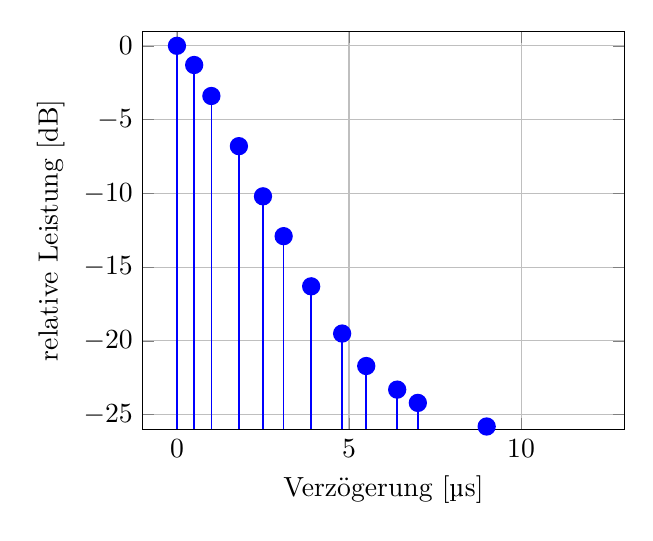
\begin{tikzpicture}
\begin{axis}[
xlabel={Verzögerung [\textmu s]},
ylabel={relative Leistung [dB]},
ymin=-26,ymax=1,
xmin=-1,xmax=13.0,
width=7.7cm,
enlarge x limits=false,
grid=major,
]
\addplot [semithick, blue, mark=*, mark size=3, mark options={solid}, only marks, forget plot]
table{
0 0
0.5 -1.3
1 -3.4
1.8 -6.8
2.5 -10.2
3.1 -12.9
3.9 -16.3
4.8 -19.5
5.5 -21.7
6.4 -23.3
7.0 -24.2
9.0 -25.8
};
\draw [semithick, blue] 
        (axis cs: 0,-26) -- (axis cs: 0,0);
        \draw [semithick, blue] 
        (axis cs: 0.5,-26) -- (axis cs: 0.5,-1.3);
        \draw [semithick, blue] 
        (axis cs: 1,-26) -- (axis cs: 1,-3.4);
        \draw [semithick, blue] 
        (axis cs: 1.8,-26) -- (axis cs: 1.8,-6.8);
        \draw [semithick, blue] 
        (axis cs: 2.5,-26) -- (axis cs: 2.5,-10.2);
        \draw [semithick, blue] 
        (axis cs: 3.1,-26) -- (axis cs: 3.1,-12.9);
        \draw [semithick, blue] 
        (axis cs: 3.9,-26) -- (axis cs: 3.9,-16.3);
        \draw [semithick, blue] 
        (axis cs: 4.8,-26) -- (axis cs: 4.8,-19.5);
        \draw [semithick, blue] 
        (axis cs: 5.5,-26) -- (axis cs: 5.5,-21.7);
        \draw [semithick, blue] 
        (axis cs: 6.4,-26) -- (axis cs: 6.4,-23.3);
        \draw [semithick, blue] 
        (axis cs: 7,-26) -- (axis cs: 7,-24.2);
        \draw [semithick, blue] 
        (axis cs: 9,-26) -- (axis cs: 9,-25.8);
\end{axis}
\end{tikzpicture}
\caption{PDP von MR100}
        \label{plot:pdp_dvb}
    \end{minipage}% <- sonst wird hier ein Leerzeichen eingefügt
    \hfill
    \begin{minipage}[t]{0.48\textwidth}
        \centering

% PDP DAB
\begin{tikzpicture}
\begin{axis}[
xlabel={Verzögerung [\textmu s]},
xtick={,40, 80, 120, 160},
ymin=-26,ymax=1,
width=7.7cm,
ylabel near ticks, yticklabel pos=right,
xmin=-10,xmax=170.0,
enlarge x limits=false,
grid=major,
]
\addplot [semithick, magenta, mark=*, mark size=3, mark options={solid}, only marks, forget plot]
table{
0 0
80 -2
160 -3
};
\draw [semithick, magenta] 
        (axis cs: 0,-26) -- (axis cs: 0,0);
\draw [semithick, magenta] 
        (axis cs: 80,-26) -- (axis cs: 80,-2);
\draw [semithick, magenta] 
        (axis cs: 160,-26) -- (axis cs: 160,-3);
\end{axis}
\end{tikzpicture}
\caption{PDP von DAB\_HT\_2}
        \label{plot:pdp_dab}
    \end{minipage}
\end{figure}

\subsection{Kohärenzbandbreite}
Durch die verschiedenen Kanallaufzeiten der einzelnen Mehrwege kommt es am Empfänger zu konstruktiver und destruktiver Interferenz, die von der Verzögerung der Mehrwege, aber auch von der Frequenz abhängt. In einem Frequenzband der Bandbreite B variiert deshalb die mittlere empfangene Leistung über der Frequenz, was als frequenzselektives Fading bezeichnet wird. Die Bandbreite, in der ein Kanal als flach angenommen werden kann, wird als Kohärenzbandbreite bezeichnet. Für das Kanalmodell DAB\_HT\_2, das mit $T_d = 40$ \textmu s die längsten Echos enthält, ist die Kohärenzbandbreite
\begin{equation}
B_c \coloneqq \frac{1}{2 T_d} = 12,5 \text{kHz} < 1536 \text{kHz} = B
\end{equation}

Das Gesamtübertragungssystem ist also frequenzselektiv. Durch die parallele Übertragung in OFDM Unterträgern mit der Unterträgerbreite $\Delta f = 1 \text{kHz} < 12,5 \text{kHz} = B_c$ kann jedoch jeder Unterträger als frequenzflach angenommen werden.

\subsection{Doppler-Spread}
Für die Wahl der maximalen Dopplerverschiebung wird die Geschwindigkeit eines mobilen Empfängers betrachtet. Bei einer typischen Trägerfrequenz für die terrestrische DAB Übertragung $f_T=200$ MHz ergibt sich eine Proportionalität zwischen der Geschwindigkeit und der Dopplerverschiebung.
\begin{equation}
|\Delta f_{D}| \leq f_T \frac{v}{c} = \frac{200\, \text{MHz}}{3\cdot 10^8\, \text{m/s}}\; v
\end{equation}
Der Doppler-Spread ist die maximale Differenz der auftretenden Doppler-Verschiebungen \cite{proakis}.
\begin{equation}
D_s = \max_{i,k} |\Delta f_{D,1} - \Delta f_{D,2}| = 2 |\Delta f_{D,max}|
\end{equation}
Die folgenden Dopplerverschiebungen und damit korrespondierenden Geschwindigkeiten werden untersucht:

\begin{figure} [h]
\begin{center}
\begin{tabular}{c | c | l}
$|\Delta f_{D,max}|$ [Hz] & $v$ [km/h] & Bewegungsprofil \\
\hline
5 & 27 & Fahrt in Wohngebiet \\
10 & 54 & Fahrt auf Hauptstraße \\
20 & 100 & Fahrt auf Autobahn \\
50 & 270 & Grenzwert für maximale Geschwindigkeit
\end{tabular}
\caption{Untersuchte Bewegungsprofile}
\label{tab:doppler_werte}
\end{center}
\end{figure}

\subsubsection{Kohärenzzeit}
Die Kohärenzzeit definiert die Zeitspanne, in welcher sich der Kanal nicht nennenswert ändert. Die Kohärenzzeit berechnet sich aus dem Doppler-Spread.
\begin{equation}
T_{c} \coloneqq \frac{1}{4 D_s} \geq \frac{1}{4 D_{s,max}} = 2,5\, \text{ms} > 1\, \text{ms} = T_s
\end{equation}
Da selbst für den größten hier betrachteten Doppler-Spread die Kohärenzzeit größer als die Symboldauer ist, liegt in allen betrachteten Szenarien slow fading vor, das heißt der Kanal ändert sich innerhalb der Dauer eines Symbols nicht nennenswert.

\subsection{Bitfehlerrate}
In Abb.~\ref{plot:ber_dvb} sind die Bitfehlerraten des DAB OFDM Systems über dem $\text{E}_b/\text{N}_0$ im MR100 Kanal aufgetragen. Die simulierten Doppler-Spreads entsprechen den in Tabelle \ref{tab:doppler_werte} gezeigten typischen Geschwindigkeiten. Als Referenz ist die theoretische BER Kurve eines Rayleigh-Fading Kanals bei D-QPSK Modulation mit Antennendiversität 1 abgebildet.

% BER over SNR, differnt doppler spreads, DVB + DAB
\begin{figure}[htb]
    \centering
    \begin{minipage}[t]{0.48\textwidth}
        \centering
        
        \begin{tikzpicture}
        \begin{axis}[
        ymode=log,
        xlabel={$\text{E}_b/\text{N}_0$ [dB]},
        enlarge x limits=false,
        ylabel={BER},
        ymin=0.00003,ymax=1.0,
        grid=major,
        width=7.8cm,
        legend entries={$f_{D,max}=5$Hz, $f_{D,max}=10$Hz, $f_{D,max}=20$Hz, $f_{D,max}=50$Hz, Rayleigh (theo.)},
        legend style={at={(0.05,0.05)},anchor=south west, font=\tiny},
        legend cell align={left},
        ]
        \addplot [blue, mark=diamond*]table {simulation/dynamic/BER/171118_dynamic_doppler_5.0_BER_DVB.dat};
        \addplot [green, mark=diamond*]table {simulation/dynamic/BER/171118_dynamic_doppler_10.0_BER_DVB.dat};
        \addplot [cyan, mark=diamond*]table {simulation/dynamic/BER/171118_dynamic_doppler_20.0_BER_DVB.dat};
        \addplot [magenta, mark=diamond*]table {simulation/dynamic/BER/171118_dynamic_doppler_50.0_BER_DVB.dat};
        \addplot [black, mark=o]table {simulation/dynamic/BER/171119_dynamic_doppler_theo.dat};
        \end{axis}
        \end{tikzpicture}
        
        \caption{BER für MR100}
        \label{plot:ber_dvb}
    \end{minipage}% <- sonst wird hier ein Leerzeichen eingefügt
    \hfill
    \begin{minipage}[t]{0.48\textwidth}
        \centering
        
        \begin{tikzpicture}
        \begin{axis}[
        ymode=log,
        xlabel={$\text{E}_b/\text{N}_0$ [dB]},
        enlarge x limits=false,
        grid=major,
        width=7.8cm,
        ylabel near ticks, yticklabel pos=right,
        ymin=0.00003,ymax=1.0,
        legend entries={$f_{D,max}=1$Hz, $f_{D,max}=5$Hz, $f_{D,max}=10$Hz, $f_{D,max}=20$Hz, $f_{D,max}=50$Hz},
        legend style={at={(0.05,0.05)},anchor=south west, font=\tiny},
        legend cell align={left},
        ]
        \addplot [brown, mark=diamond*]table {simulation/dynamic/BER/171114_dynamic_doppler_1.0_BER.dat};
        \addplot [blue, mark=diamond*]table {simulation/dynamic/BER/171114_dynamic_doppler_5.0_BER.dat};
        \addplot [green, mark=diamond*]table {simulation/dynamic/BER/171114_dynamic_doppler_10.0_BER.dat};
        \addplot [cyan, mark=diamond*]table {simulation/dynamic/BER/171114_dynamic_doppler_20.0_BER.dat};
        \addplot [magenta, mark=diamond*]table {simulation/dynamic/BER/171114_dynamic_doppler_50.0_BER.dat};
        \end{axis}
        \end{tikzpicture}
        
        \caption{BER für DAB\_HT\_2}
        \label{plot:ber_dab_ht}
    \end{minipage}
\end{figure}


Im Vergleich zur theoretischen BER Kurve im AWGN Kanal (Abb.~\ref{plot:awgn_ber}), schneidet die BER im Rayleigh-Fading Kanal deutlich schlechter ab. Die Simulationsergebnisse für geringe Dopplerverschiebungen liegen nahe an der theoretischen Kurve. Mit zunehmendem Doppler-Spread laufen die Kurven immer früher in einen Error-Floor. Sehr schlechte Ergebnisse liefert eine Simulation mit der maximalen Dopplerverschiebung von 50Hz. Eine BER von unter $10^{-2}$ wird selbst bei hohem SNR nicht erreicht.
\\
In Abb.~\ref{plot:ber_dab_ht} sind die Ergebnisse der BER Simulation für das Kanalmodell DAB\_HT\_2 dargestellt. Die BER Kurven haben den gleichen Verlauf wie die Kurven in Abb.~\ref{plot:ber_dvb} und sind um etwa 3 dB nach rechts verschoben. Die BER für 50 Hz Dopplerverschiebung läuft außerdem in einen schlechteren Error-Floor von etwa $5\cdot 10^{-2}$. Die geringe Verschlechterung im Kanalmodell DAB\_HT\_2 im Vergleich zu MR100 demonstriert die Robustheit des DAB Systems gegen stark verzögerte Mehrwege. Die CP Länge von $T_B =$ 246 \textmu s ist dabei noch nicht ausgereizt.\\

\subsection{Paketfehlerrate}
Die Paketfehlerrate im Rayleigh-Fading Kanal mit realistischem PDP bildet schließlich die Simulation, die der subjektiven Empfangsqualität im Realfall am nächsten kommt. Wegen der Ähnlichkeit von den BER Kurven der beiden Kanalmodelle, wurde die PER nur für das Kanalmodell DAB\_HT\_2 untersucht. Die Simulationsergebenisse sind in Abb.~\ref{plot:doppler_per} gezeigt.

% PER doppler
\begin{figure}[htb]
\begin{center}
\begin{tikzpicture}
\begin{axis}[
ymode=log,
xlabel={$\text{E}_b/\text{N}_0$ [dB]},
ylabel={PER},
ymin=0.0001,ymax=1.0,
xmin=5.0,xmax=35.0,
enlarge x limits=false,
grid=major,
legend entries={$f_{D,max}=5$Hz, $f_{D,max}=10$Hz, $f_{D,max}=20$Hz, $f_{D,max}=50$Hz},
        legend style={at={(0.05,0.05)},anchor=south west, font=\tiny},
        legend cell align={left},
]
\addplot [blue, mark=diamond*]table {simulation/dynamic/PER/171116_dynamic_doppler_5.0_FIC.dat};
\addplot [green, mark=diamond*]table {simulation/dynamic/PER/171115_dynamic_doppler_10.0_FIC.dat};
\addplot [cyan, mark=diamond*]table {simulation/dynamic/PER/171116_dynamic_doppler_20.0_FIC.dat};
\addplot [magenta, mark=diamond*]table {simulation/dynamic/PER/171120_dynamic_doppler_50.0_FIC.dat};
\end{axis}
\end{tikzpicture}
\end{center}
\caption{PER für DAB\_HT\_2}
\label{plot:doppler_per}
\end{figure}

Die PER Kurven für maximale Dopplerverschiebungen von 5 - 20 Hz weisen deutlich bessere Werte als die entsprechenden BER Kurven auf und sind sehr zufriedenstellend. Die Kanalcodierung trägt hier einen enormen Teil durch die Fehlerkorrektur bei. Lediglich die PER mit einer maximalen Dopplerverschiebung von 50Hz verbessert sich durch die Kanalcodierung nicht signifikant und läuft in einen Error-Floor mit einer PER von $3 \cdot 10^{-2}$. Es treten zu viele Bitfehler auf, wodurch die Korrekturwahrscheinlichkeit des Faltungscodes sehr gering ist. Die Dopplerverschiebung von 50 Hz entspricht einer Geschwindigkeit von 270 km/h. Der Wert wurde bewusst sehr hoch angesetzt um die Grenzen des Systems zu testen. PERs mit Werten über $10^{-2}$ stellen eine ungenügende Empfangsqualität dar. Eine tatsächliche Grenze für ausreichenden Empfang ist daher zwischen 20 Hz und 50 Hz anzusetzten.